\documentclass[usenames]{beamer}

\mode<presentation>
{
%  \usetheme{Hannover}
\usetheme[width=0.7in]{Hannover}
% or ...

  \setbeamercovered{transparent}
  % or whatever (possibly just delete it)
}

\usepackage{times}
\usepackage{tikz}
\usetikzlibrary{positioning}

\usepackage{hyperref}

\hypersetup{colorlinks=true,
    linkcolor=blue,
    citecolor=blue,
    filecolor=blue,
    urlcolor=blue,
    unicode=false}

\usepackage{totpages}
\usepackage[round]{natbib}

\usepackage{listings}
\lstset{frame=none, showstringspaces=false, basicstyle=\ttfamily\bfseries\footnotesize,
  xleftmargin=-8mm,language=Haskell,breaklines=true}

\pgfdeclareimage[height=0.7cm]{logo}{../figures/McMasterLogo}
\title[\pgfuseimage{logo}] {Sustainable Software Product Lines via Generation}

\author[Smith \& Carette,\\Slide \thepage~of \pageref{TotPages}]{\textbf{Spencer
Smith} and Jacques Carette}

\institute[McMaster University]
{
  Computing and Software Department\\
  Faculty of Engineering\\
  McMaster University
}

\date {Huawei 2023 Visit: Feb?, 2023}

\subject{research software, software engineering, software
  quality, code and artifact generation, software documentation}
% This is only inserted into the PDF information catalog. Can be left
% out. 

\beamertemplatenavigationsymbolsempty 

\begin{document}

%%%%%%%%%%%%%%%%%%%%%%%%%%%%%%%%%%%%%%

\hoffset=-.4in %removing side bar for these frames
\begin{frame}[plain]

\titlepage

\end{frame}
\hoffset=0in %restore

%%%%%%%%%%%%%%%%%%%%%%%%%%%%%%%%%%%%%%

\begin{frame}

\frametitle{Generate All Things with Drasil}

\begin{itemize}
\item \textbf{Goal} --- Improve software sustainability and productivity
\item \textbf{Ideas}
  \begin{itemize}
  \item Adapt a software product line approach 
  \item Build on success of MDSE
  \item Value all documents, not just code
  \item Start with well-understood domains
  \end{itemize}
\item \textbf{Solution}
\begin{itemize}
\item Capture (codify) knowledge \textcolor{red}{once}
\item Generate all \textcolor{red}{documentation} and code
\item Idealized dev process for \textcolor{red}{well-understood} software
\end{itemize}
\item \textbf{Implement Partial Solution ---
    \href{https://github.com/JacquesCarette/Drasil} {Drasil}}
\end{itemize}

\end{frame}

%%%%%%%%%%%%%%%%%%%%%%%%%%%%%%%%%%%%%%

\section[Introduction]{Introduction}

%%%%%%%%%%%%%%%%%%%%%%%%%%%%%%%%%%%%%%

%\hoffset=-.8in
\begin{frame}[plain, fragile]

\frametitle{Product Lines}

% if time add another program family example

\begin{tikzpicture}[remember picture,overlay]
\node [xshift=0cm,yshift=-3.cm] at (current page.center)
{
\includegraphics[width=1.2\textwidth]{../../CSE_2016/apple-mac-products-450x128.jpg}
};
\end{tikzpicture}

\begin{tikzpicture}[remember picture,overlay]
\node [xshift=0cm,yshift=1.cm] at (current page.center)
{
\includegraphics[width=0.8\textwidth]{../../CSE_2016/dodge-lineup.jpg}
};
\end{tikzpicture}

% product line when economically makes sense to dev together
% advantages of product line approach:
% reduced dev time
% improved quality
% improved reusability
% improved modifiability for likely changes

\end{frame}
%\hoffset=0in

%%%%%%%%%%%%%%%%%%%%%%%%%%%%%%%%%%%%%%

\begin{frame}[plain, fragile]

\frametitle{Product Lines in User Manual}

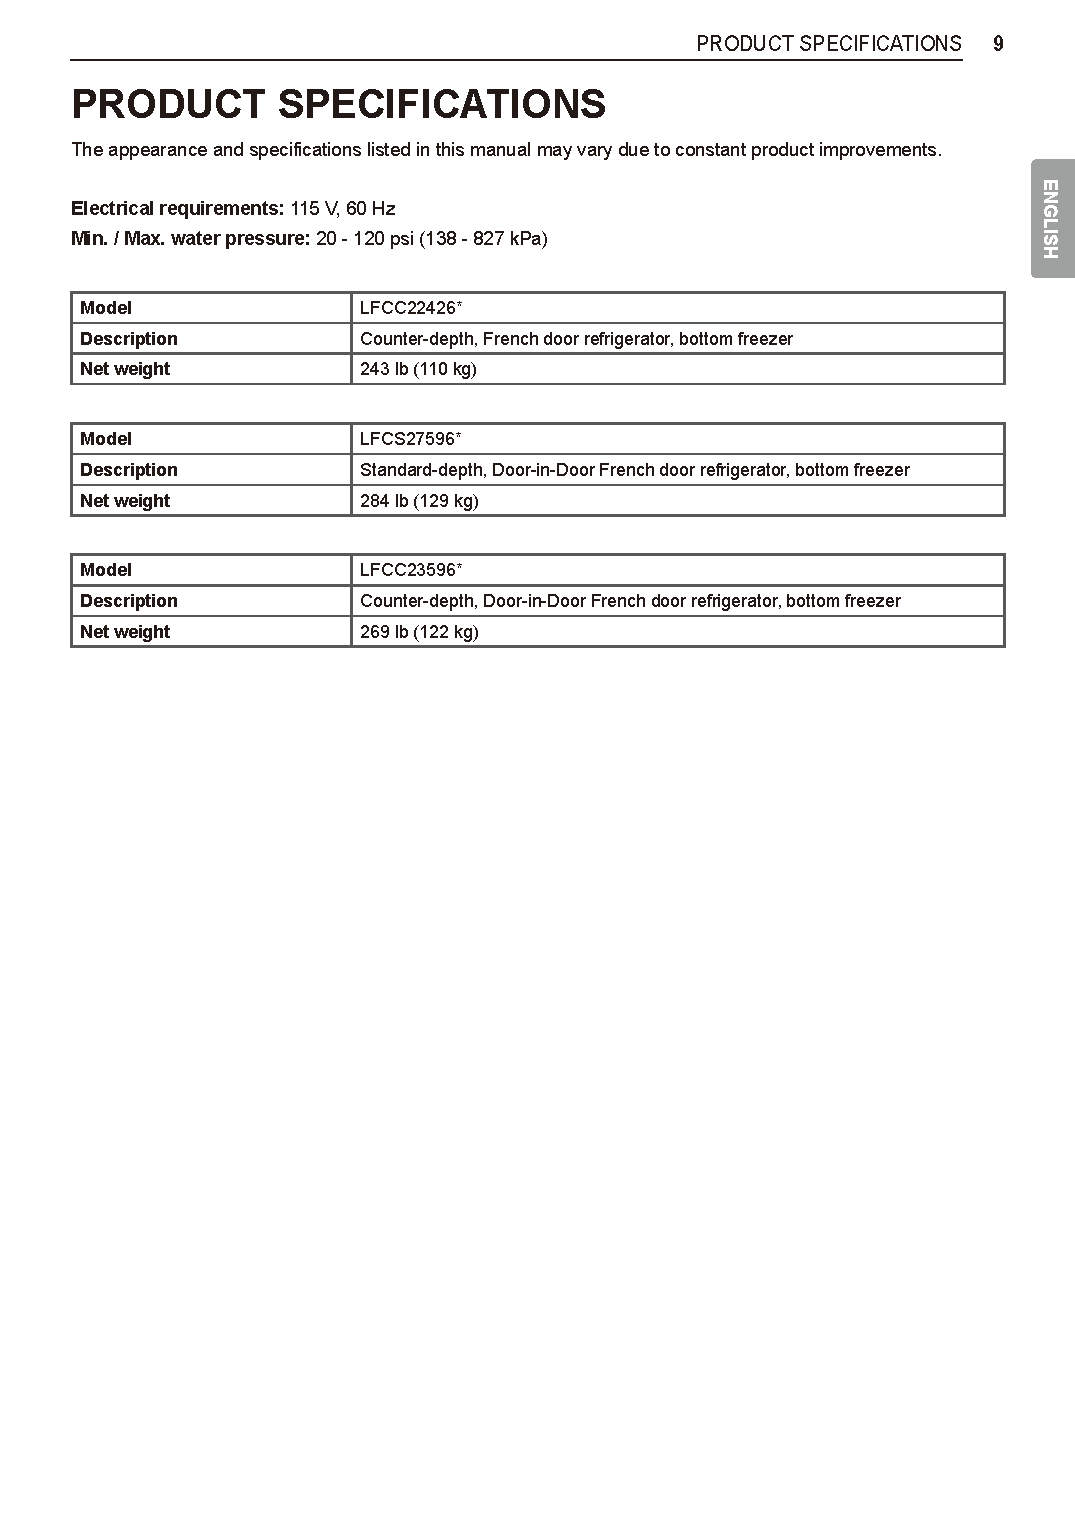
\includegraphics[width=0.95\textwidth]{../figures/FrigFamily.pdf}

% common to see all products in the same manual
% online version for different languages, but not for different products
% may vary due to product improvements (not integrated)
\end{frame}

%%%%%%%%%%%%%%%%%%%%%%%%%%%%%%%%%%%%%%

\begin{frame}[plain, fragile]

%\frametitle{Model-Based Product Line}

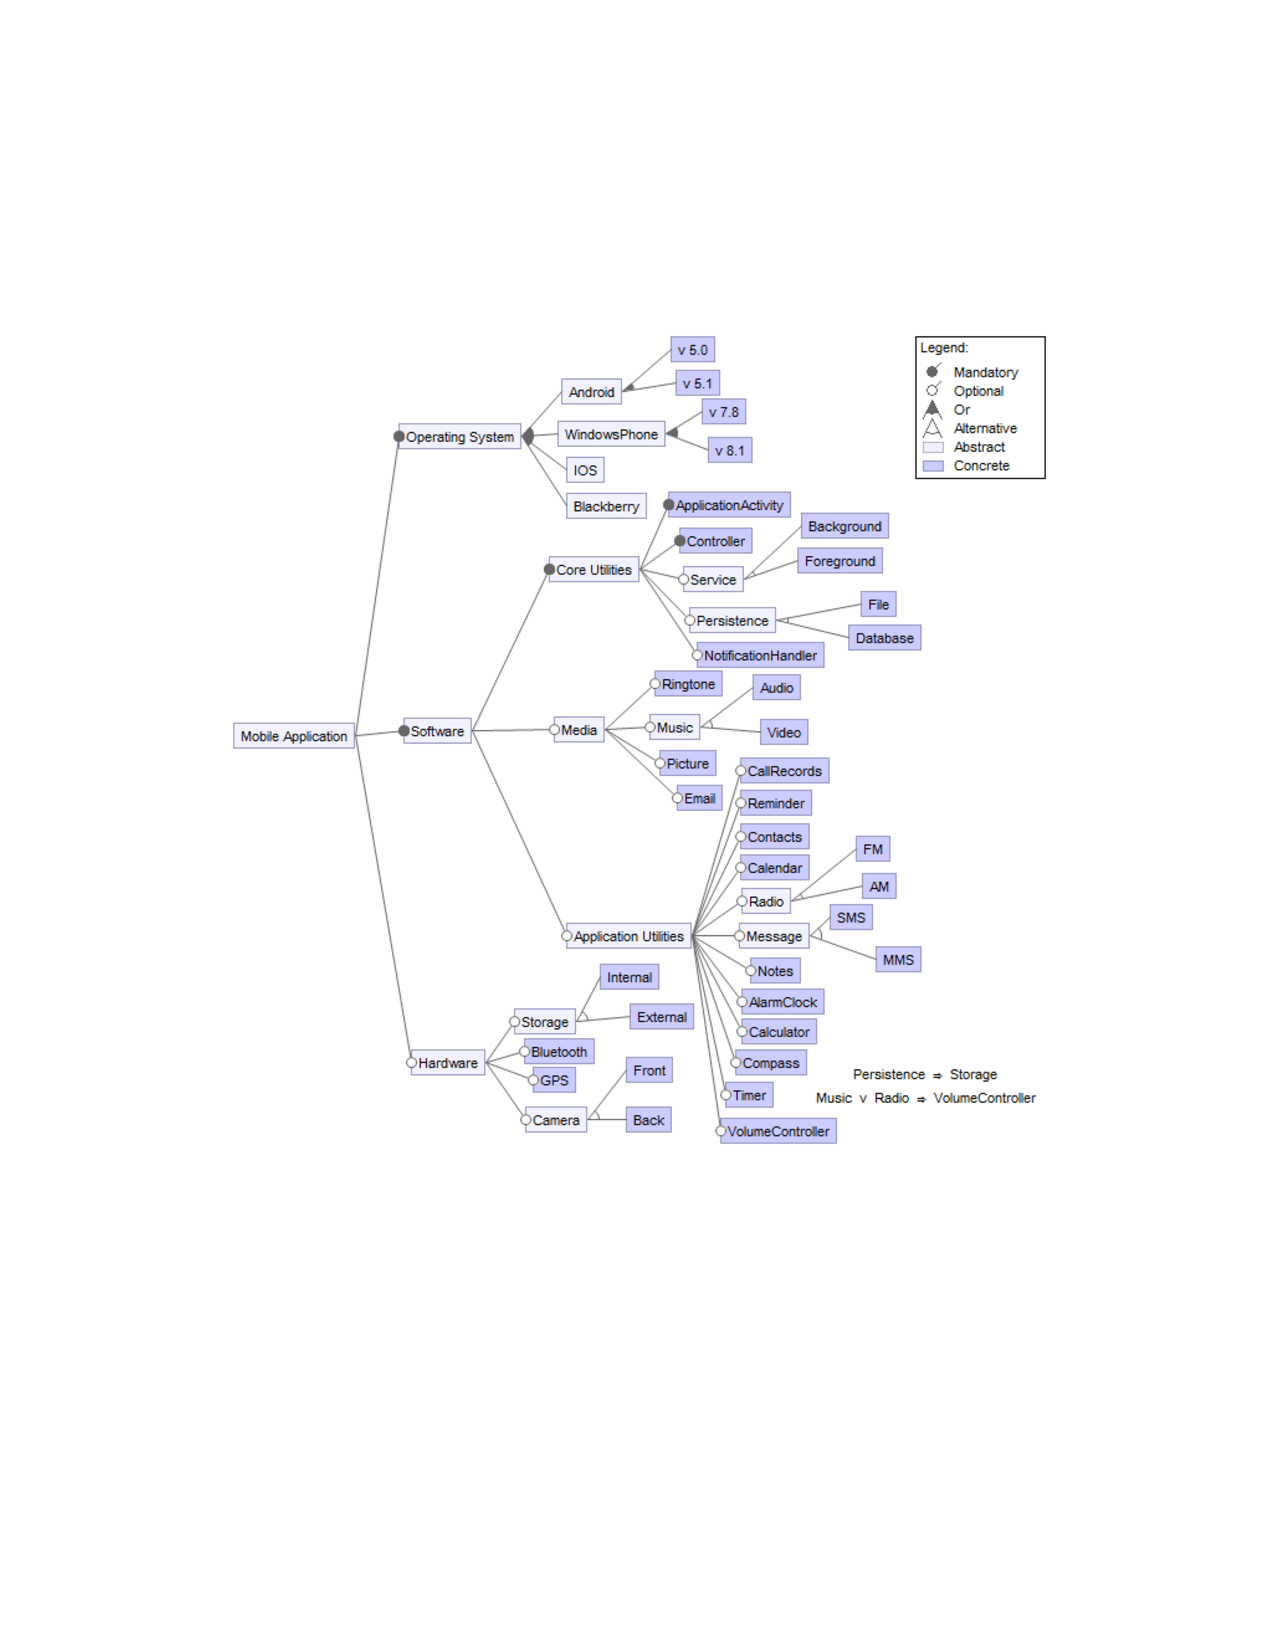
\includegraphics[width=0.85\textwidth]{../figures/MobileAppFeatureModel.pdf}

\citet{UsmanEtAl2017}

% how program family concept is realized
% tools to support product line approach
% systematic way to handle variabilities
% generate code for family members
\end{frame}

%%%%%%%%%%%%%%%%%%%%%%%%%%%%%%%%%%%%%%

\begin{frame}

\frametitle{Build on Success of MDSE}

\begin{itemize}
  \item Codify (capture) code and non-code info together
  \begin{itemize}
    \item Natural language (text)
    \item Definitions
    \item Assumptions
    \item Derivations
    \item Rationale
    \item Abstract theory
    \item User characteristics
    \item Nonfunctional Requirements
    \item Etc.
  \end{itemize}
\item Generate all artifacts from one framework
\begin{itemize}
  \item Requirements
  \item User manuals
  \item README
  \item Build scripts, dev environment (CI etc)
  \item Assurance case
  \item Code (in different languages)
  \item Test cases
  \item etc.
\end{itemize}
\end{itemize}

\end{frame}

%%%%%%%%%%%%%%%%%%%%%%%%%%%%%%%%%%%%%%
\hoffset=-.4in
\begin{frame}[plain, fragile]

%\frametitle{Generate All Things}

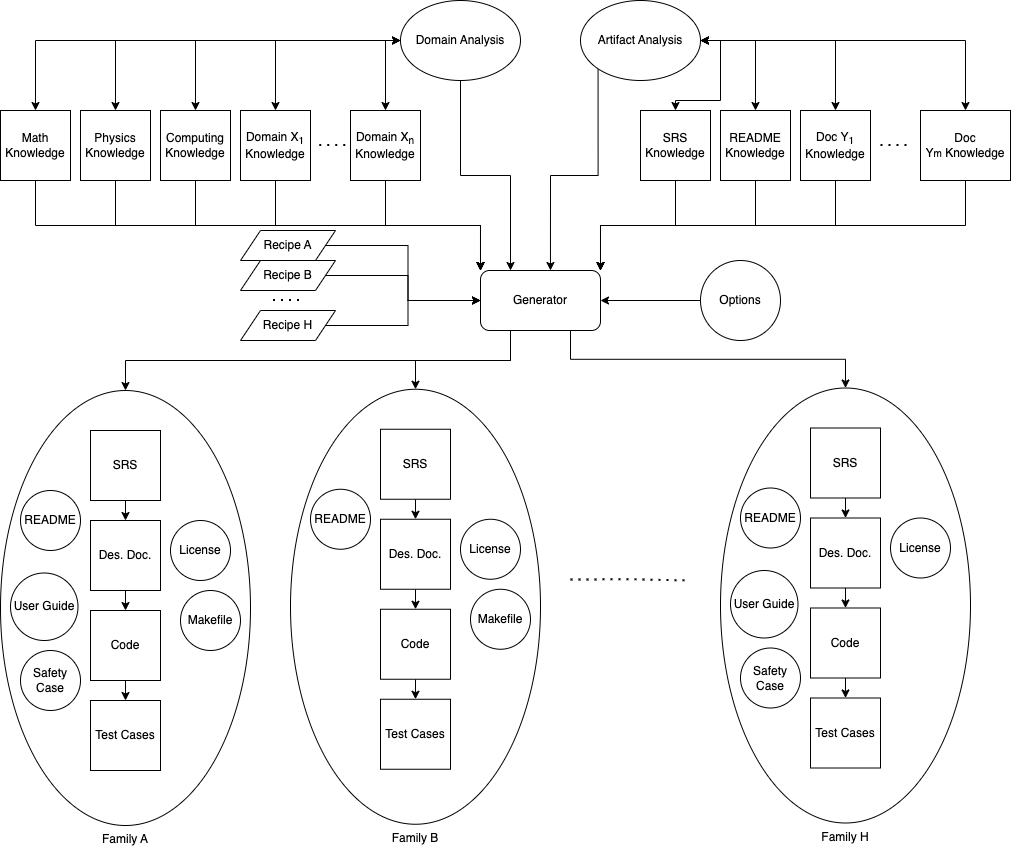
\includegraphics[width=1.05\textwidth]{../figures/GenAllThings.png}

\end{frame}
\hoffset=0in 
%%%%%%%%%%%%%%%%%%%%%%%%%%%%%%%%%%%%%%

\begin{frame}

\frametitle{Why Generate All Things?}

\begin{itemize}
\item Different views of the same knowledge
\item Generate the view needed by the audience
\item Change to different natural languages
\item Stay abstract longer
\item Certification
\item Documentation improve productivity, sustainability
\item Reusability
\item Modifiability
\item One source helps synchronization
\end{itemize}

\end{frame}

%%%%%%%%%%%%%%%%%%%%%%%%%%%%%%%%%%%%%%

\section[GlassBR Example]{GlassBR Example}

%%%%%%%%%%%%%%%%%%%%%%%%%%%%%%%%%%%%%%

\begin{frame}

\frametitle{GlassBR}

\begin{columns}
\begin{column}{0.5\textwidth}
\includegraphics[width=1.0\textwidth]{../figures/physicalsystimage.png}
\end{column}
\begin{column}{0.5\textwidth}
Given

\begin{itemize}
\item dimensions of glass plane
\item glass type
\item explosion characteristics
\item tolerable breakage probability
\end{itemize}

Predict whether the glass will withstand the explosion

\end{column}
\end{columns}

\end{frame}

%%%%%%%%%%%%%%%%%%%%%%%%%%%%%%%%%%%%%%

\begin{frame}

%\frametitle{Input Knowledge}

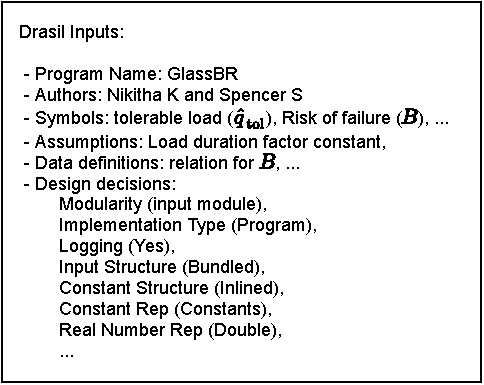
\includegraphics[width=0.95\textwidth]{../figures/DrasilInputs.pdf}

\end{frame}

%%%%%%%%%%%%%%%%%%%%%%%%%%%%%%%%%%%%%%

\begin{frame}

%\frametitle{Input Knowledge}

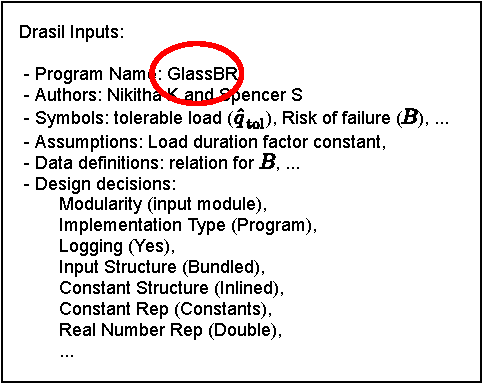
\includegraphics[width=0.95\textwidth]{../figures/InputsCircleGlassBR.pdf}

\end{frame}

%%%%%%%%%%%%%%%%%%%%%%%%%%%%%%%%%%%%%%
\hoffset=-.4in
\begin{frame}[plain, fragile]

%\frametitle{Input Knowledge}

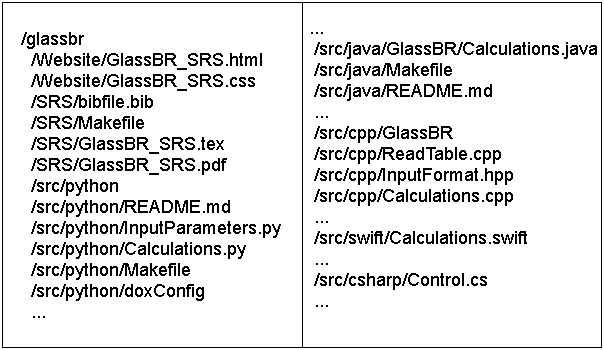
\includegraphics[width=1.05\textwidth]{../figures/FoldersFiles.pdf}

\end{frame}
\hoffset=0in
%%%%%%%%%%%%%%%%%%%%%%%%%%%%%%%%%%%%%%
\hoffset=-.4in
\begin{frame}[plain, fragile]

%\frametitle{Input Knowledge}

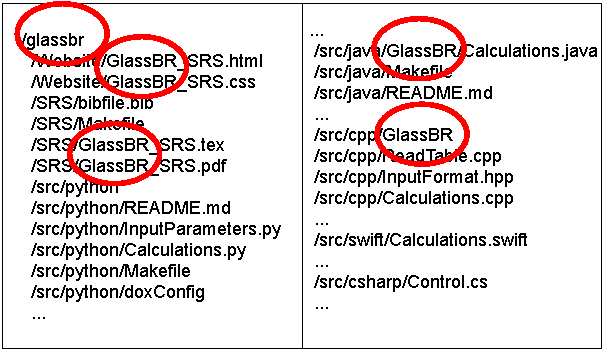
\includegraphics[width=1.05\textwidth]{../figures/FoldersFilesCircleGlassBR.pdf}

\end{frame}
\hoffset=0in
%%%%%%%%%%%%%%%%%%%%%%%%%%%%%%%%%%%%%%
\hoffset=-.4in
\begin{frame}[plain, fragile]

%\frametitle{Input Knowledge}

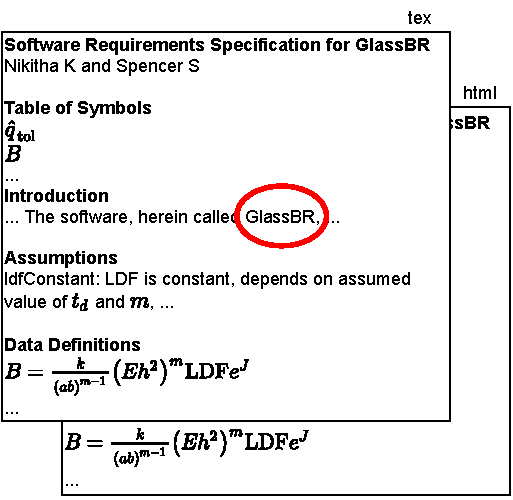
\includegraphics[width=1.02\textwidth]{../figures/SRSCircleGlassBR.pdf}

\end{frame}
\hoffset=0in
%%%%%%%%%%%%%%%%%%%%%%%%%%%%%%%%%%%%%%
\hoffset=-.4in
\begin{frame}[plain, fragile]

%\frametitle{Input Knowledge}

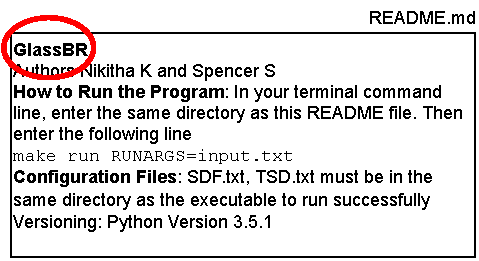
\includegraphics[width=1.05\textwidth]{../figures/READMECircleGlassBR.pdf}

\end{frame}
\hoffset=0in
%%%%%%%%%%%%%%%%%%%%%%%%%%%%%%%%%%%%%%
\hoffset=-.4in
\begin{frame}[plain, fragile]

%\frametitle{Input Knowledge}

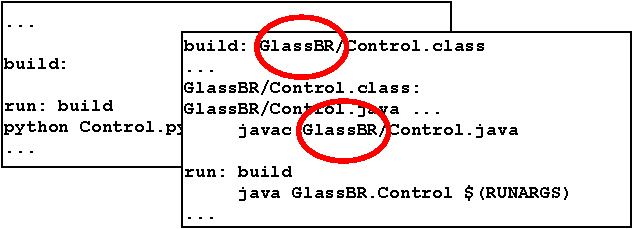
\includegraphics[width=1.05\textwidth]{../figures/MakefileCircleGlassBR.pdf}

\end{frame}
\hoffset=0in
%%%%%%%%%%%%%%%%%%%%%%%%%%%%%%%%%%%%%%
\hoffset=-.4in
\begin{frame}[plain, fragile]

%\frametitle{Input Knowledge}

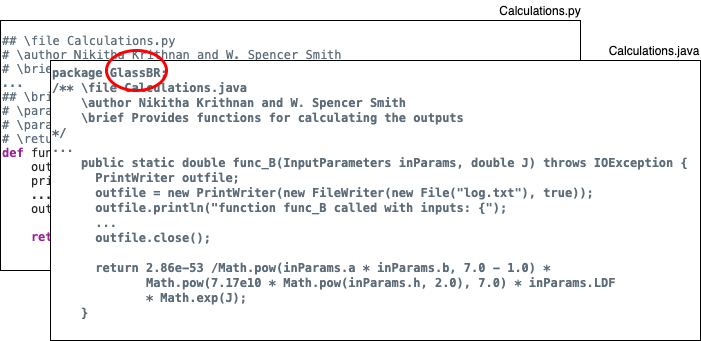
\includegraphics[width=1.05\textwidth]{../figures/CodeCircleGlassBR.png}

\end{frame}
\hoffset=0in
%%%%%%%%%%%%%%%%%%%%%%%%%%%%%%%%%%%%%%

\begin{frame}

\frametitle{$J_{\mbox{tol}}$ in SRS.pdf}
\begin{center}
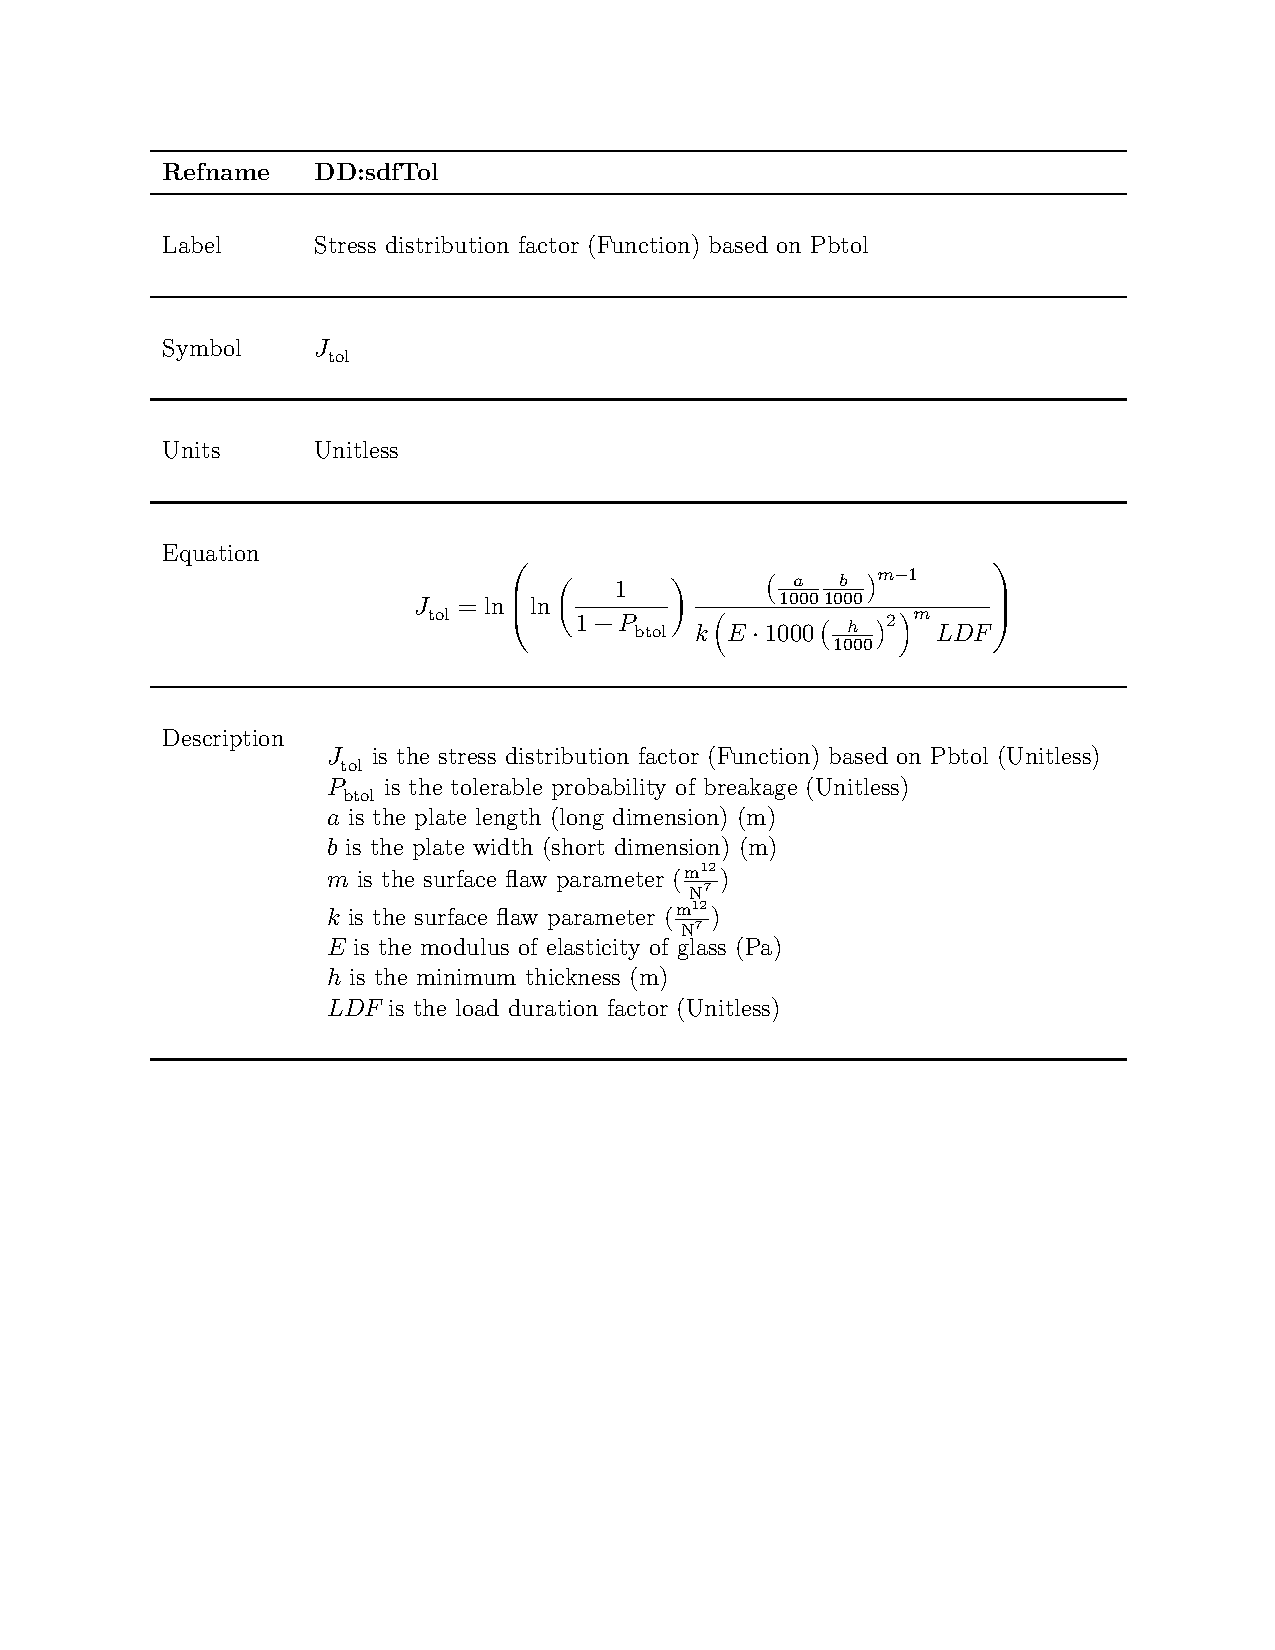
\includegraphics[width=0.9\textwidth]{../figures/Jtol_pdf.pdf}
\end{center}
\end{frame}

%%%%%%%%%%%%%%%%%%%%%%%%%%%%%%%%%%%%%
\hoffset=-.3in
\begin{frame}[plain, fragile]

\frametitle{$J_{\mbox{tol}}$ in SRS.tex}
~\\
\begin{lstlisting}
...
Label & Stress distribution factor (Function) based on Pbtol
        
\\ \midrule \\
Symbol & ${J_{\text{tol}}}$
         
\\ \midrule \\
Units & Unitless
        
\\ \midrule \\
Equation & \begin{displaymath}
           {J_{\text{tol}}}=\ln\left(\ln\left(\frac{1}{1-{P_{\text{b}\text{tol}}}}\right) \frac{\left(\frac{a}{1000} \frac{b}{1000}\right)^{m-1}}{k \left(E\cdot{}1000 \left(\frac{h}{1000}\right)^{2}\right)^{m} LDF}\right)
           \end{displaymath}
\\ \midrule \\
Description & ...
\end{lstlisting}
\end{frame}
\hoffset=0in
%%%%%%%%%%%%%%%%%%%%%%%%%%%%%%%%%%%%%%
\hoffset=-.3in
\begin{frame}[plain, fragile]

\frametitle{$J_{\mbox{tol}}$ in SRS.html}

\begin{lstlisting}

...
<th>Equation</th>
<td>
\[{J_{\text{tol}}}=\ln\left(\ln\left(\frac{1}{1-{P_{\text{b}\text{tol}}}}\right) \frac{\left(\frac{a}{1000} \frac{b}{1000}\right)^{m-1}}{k \left(E\cdot{}1000 \left(\frac{h}{1000}\right)^{2}\right)^{m} LDF}\right)\]
</td>
...
\end{lstlisting}

\end{frame}
\hoffset=0in
%%%%%%%%%%%%%%%%%%%%%%%%%%%%%%%%%%%%%
\hoffset=-.3in
\begin{frame}[plain, fragile]

\frametitle{$J_{\mbox{tol}}$ in Python}

\begin{lstlisting}
## \brief Calculates stress distribution factor (Function) based on Pbtol
# \param inParams structure holding the input values
# \return stress distribution factor (Function) based on Pbtol
def func_J_tol(inParams):
    outfile = open("log.txt", "a")
    print("function func_J_tol called with inputs: {", file=outfile)
    print("  inParams = ", end="", file=outfile)
    print("Instance of InputParameters object", file=outfile)
    print("  }", file=outfile)
    outfile.close()
    
    return math.log(math.log(1.0 / (1.0 - inParams.P_btol)) * ((inParams.a / 1000.0 * (inParams.b / 1000.0)) ** (7.0 - 1.0) / (2.86e-53 * (7.17e10 * 1000.0 * (inParams.h / 1000.0) ** 2.0) ** 7.0 * inParams.LDF)))
\end{lstlisting}
\end{frame}
\hoffset=0in
%%%%%%%%%%%%%%%%%%%%%%%%%%%%%%%%%%%%%%
\hoffset=-.3in
\begin{frame}[plain, fragile]

\frametitle{$J_{\mbox{tol}}$ in Java}

\begin{lstlisting}
    /** \brief Calculates stress distribution factor (Function) based on Pbtol
        \param inParams structure holding the input values
        \return stress distribution factor (Function) based on Pbtol
    */
    public static double func_J_tol(InputParameters inParams) throws IOException {
        PrintWriter outfile;
        outfile = new PrintWriter(new FileWriter(new File("log.txt"), true));
        ...
        return Math.log(Math.log(1.0 / (1.0 - inParams.P_btol)) * (Math.pow(inParams.a / 1000.0 * (inParams.b / 1000.0), 7.0 - 1.0) / (2.86e-53 * Math.pow(7.17e10 * 1000.0 * Math.pow(inParams.h / 1000.0, 2.0), 7.0) * inParams.LDF)));
    }
\end{lstlisting}
\end{frame}
\hoffset=0in
%%%%%%%%%%%%%%%%%%%%%%%%%%%%%%%%%%%%%%
\hoffset=-.3in
\begin{frame}[plain, fragile]

\frametitle{$J_{\mbox{tol}}$ in Drasil (Haskell)}

\begin{lstlisting}

tolStrDisFacEq :: Expr
tolStrDisFacEq = ln (ln (recip_ (exactDbl 1 $- sy pbTol))
  `mulRe` (((sy plateLen $/ exactDbl 1000) `mulRe` (sy plateWidth $/ exactDbl 1000)) $^ (sy sflawParamM $- exactDbl 1) $/
    (sy sflawParamK `mulRe` ((sy modElas `mulRe` exactDbl 1000 `mulRe`
    square (sy minThick $/ exactDbl 1000)) $^ sy sflawParamM) `mulRe` sy lDurFac)))

\end{lstlisting}
\end{frame}
\hoffset=0in
%%%%%%%%%%%%%%%%%%%%%%%%%%%%%%%%%%%%%%
\hoffset=-.3in
\begin{frame}[plain, fragile]

\frametitle{$J_{\mbox{tol}}$ without Unit Conversion}

\begin{lstlisting}
tolStrDisFacEq :: Expr
tolStrDisFacEq = ln (ln (recip_ (exactDbl 1 $- sy pbTol))
  `mulRe` ((sy plateLen `mulRe` sy plateWidth) $^ (sy sflawParamM $- exactDbl 1) $/
    (sy sflawParamK `mulRe` ((sy modElas `mulRe`
    square (sy minThick)) $^ sy sflawParamM) `mulRe` sy lDurFac)))
\end{lstlisting}
\end{frame}
\hoffset=0in
%%%%%%%%%%%%%%%%%%%%%%%%%%%%%%%%%%%%%%

\begin{frame}

%\frametitle{Input Knowledge}

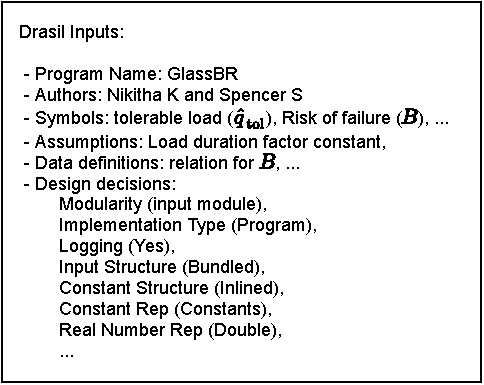
\includegraphics[width=0.95\textwidth]{../figures/DrasilInputs.pdf}

\end{frame}

%%%%%%%%%%%%%%%%%%%%%%%%%%%%%%%%%%%%%%
\hoffset=-0.4in
\begin{frame}[plain, fragile]

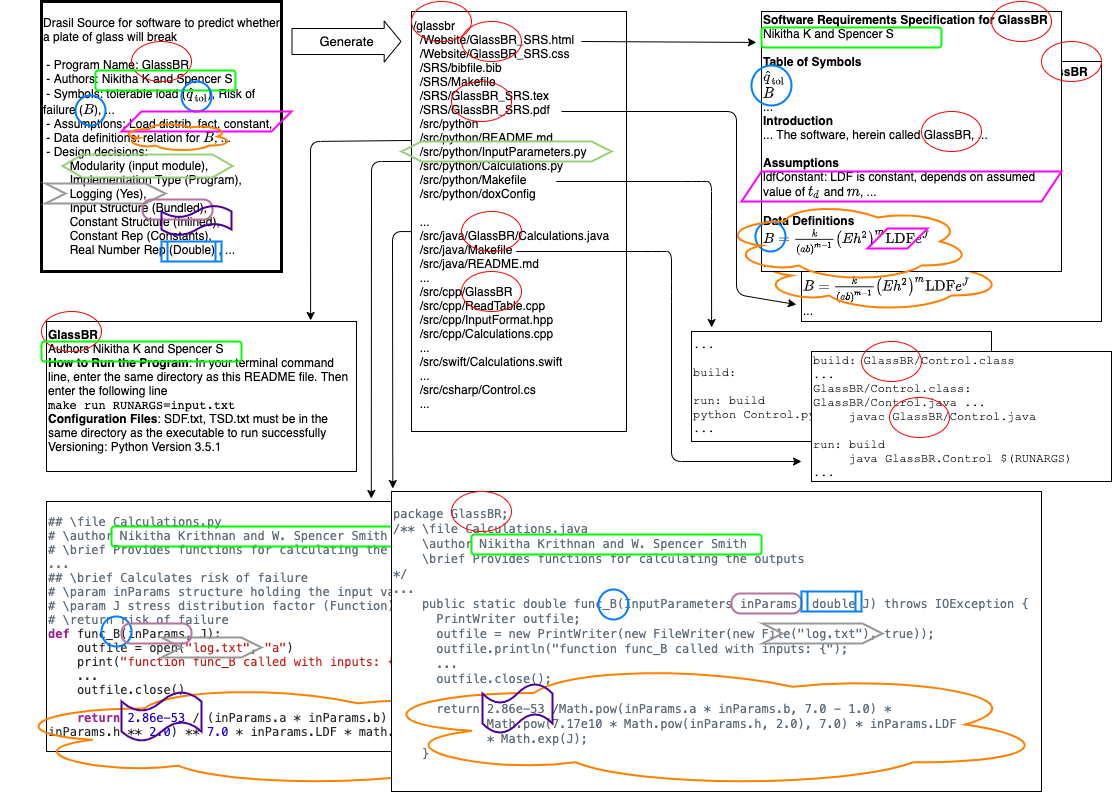
\includegraphics[width=1.08\textwidth]{../figures/DrasilSupportsChange.png}

\end{frame}
\hoffset=0in
%%%%%%%%%%%%%%%%%%%%%%%%%%%%%%%%%%%%%%

\section[Idealized Process]{Idealized Process}

%%%%%%%%%%%%%%%%%%%%%%%%%%%%%%%%%%%%%%

\begin{frame}

\frametitle{Idealized Process}

\begin{itemize}
\item From wu paper
\end{itemize}

\end{frame}

%%%%%%%%%%%%%%%%%%%%%%%%%%%%%%%%%%%%%%

\section[Inputs]{Capturing Knowledge: Inputs}

%%%%%%%%%%%%%%%%%%%%%%%%%%%%%%%%%%%%%%

\begin{frame}

\frametitle{Capturing Knowledge: Inputs}

\begin{itemize}
\item Probably won't have time to discuss
\end{itemize}

\end{frame}

%%%%%%%%%%%%%%%%%%%%%%%%%%%%%%%%%%%%%%

\section[Concluding Remarks]{Concluding Remarks}

%%%%%%%%%%%%%%%%%%%%%%%%%%%%%%%%%%%%%%

\begin{frame}

\frametitle{Concluding Remarks}

\begin{itemize}
\item \textbf{Take Home Message} --- Sustainability and Productivity can
potentially be improved via a Generate All Things Approach
\end{itemize}

\end{frame}

%%%%%%%%%%%%%%%%%%%%%%%%%%%%%%%%%%%%%%

\begin{frame}[allowframebreaks]
\frametitle{References}
\bibliography{Huawei}
\bibliographystyle{plainnat}
\end{frame}

%%%%%%%%%%%%%%%%%%%%%%%%%%%%%%%%%%%%%%

\begin{frame}
\frametitle{Image Credits}

\begin{itemize} 
\item \href{https://www.apple.com/ca/store} {Apple Product Line Image}
\item
\href{https://www.motorauthority.com/news/1055062_2011-chicago-auto-show-sporty-r-t-trim-returns-on-five-dodge-models}
{Dodge Lineup}
\end{itemize}

\end{frame}

%%%%%%%%%%%%%%%%%%%%%%%%%%%%%%%%%%%%%%

\end{document}